\documentclass[aspectratio=169]{beamer}

\usepackage[english]{babel}
\usepackage[T1]{fontenc} % For æ, ø and å
\usepackage[utf8]{inputenc}

\usepackage{ae,aecompl}
\usepackage{pslatex}

\usepackage[export]{adjustbox}

\usefonttheme[onlymath]{serif}

\setbeamertemplate{navigation symbols}{}

\begin{document}

%%% Introduction

\begin{frame}[plain]{}
  \vspace{3ex}
  \begin{center} \Huge \bf
    Depth of Field document
  \end{center}
  \begin{center} \Large \bf
    by Kristian L. Bjørke
  \end{center}

  {\large \bf
    Introduction:
  }

  \hspace{2em}Calculations and tables of depth of field (focus depth) and hyperfocal distance for

  \hspace{2em}various camera settings for the Sony $\alpha$\hspace{0.1em}6000 (aps-c).
  

  {\large \bf
    Parameters:
  }

  {
    \small
    \begin{table}
      \centering
      \begin{tabular}{r l}
        $H$ : & Hyperfocal distance \\
        $f$ : & Focal length ($\times 1.53$ crop factor for aps-c) \\
        $N$ : & F-number (aperature diameter $\frac{f}{N}$) \\
        $D$ : & Focus distance (distance to focus point) \\ 
        $c$ : & Circle of confusion (CoC) limit (determines acceptable sharpness) \\
        \ & $c$ = 0.036 mm used (suitable for 15x10cm print viewed at 25cm distance)
      \end{tabular}
    \end{table}
  }
\end{frame}

%%% Hyperfocal distance

\begin{frame}[plain]{}
  \vspace{3ex}
  \begin{center} \LARGE \bf
    Hyperfocal distance
  \end{center}

  \begin{columns}
  \begin{column}{0.40\textwidth}
    { \Large
      $$\mathit{H = \frac{f^2}{Nc} + f}$$
    }

    \center
    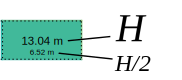
\includegraphics[width=0.80\textwidth]{img/hyperfocal-distance-example-cell.pdf}
  \end{column}
  \begin{column}{0.60\textwidth}
    \includegraphics[width=0.80\textwidth]{img/lensfocus-hyperfocal-1.pdf}

    \includegraphics[width=0.80\textwidth]{img/lensfocus-hyperfocal-2.pdf}
  \end{column}
  \end{columns}

\end{frame}

\begin{frame}[plain]{}
  \vspace{1ex}
  \centering
  Hyperfocal distance | Sony $\alpha$\hspace{0.1em}6000 (aps-c) | CoC = 0.036 mm

  \includegraphics[center,width=0.78\textwidth]{img/hyperfocal-distance.eps}
\end{frame}

%%% Depth of Field

\begin{frame}[plain]{}
  \vspace{3ex}
  \begin{center} \LARGE \bf
    Depth of Field
  \end{center}

  \begin{columns}
  \begin{column}{0.40\textwidth}
  {\Large 
    $$\mathit{d = d_1 + d_2 = \frac{2NcD^2f^2}{f^4 - N^2c^2D^2}}$$
  }

  \vspace{2ex}
  {\scriptsize
    $$\mathit{d_1 = \frac{NcD^2}{f^2 + NCD}}, \, \, \, \mathit{d_2 = \frac{NcD^2}{f^2 - NCD}}$$
  }
  \end{column}
  \begin{column}{0.60\textwidth}
    \center
    \includegraphics[width=0.90\textwidth]{img/lensfocus-dof.pdf}
  \end{column}
  \end{columns}

\end{frame}

\begin{frame}[plain]{}
  \vspace{1ex}
  \centering
  Depth of Field | {\bf Focal length = 16 mm} |  Sony $\alpha$\hspace{0.1em}6000 (aps-c) | CoC = 0.036 mm
  
  \includegraphics[center,width=0.78\textwidth]{img/depth-of-field_focl16.eps}
\end{frame}

\begin{frame}[plain]{}
  \vspace{1ex}
  \centering
  Depth of Field | {\bf Focal length = 20 mm} |  Sony $\alpha$\hspace{0.1em}6000 (aps-c) | CoC = 0.036 mm
  
  \includegraphics[center,width=0.78\textwidth]{img/depth-of-field_focl20.eps}
\end{frame}

\begin{frame}[plain]{}
  \vspace{1ex}
  \centering
  Depth of Field | {\bf Focal length = 30 mm} |  Sony $\alpha$\hspace{0.1em}6000 (aps-c) | CoC = 0.036 mm
  
  \includegraphics[center,width=0.78\textwidth]{img/depth-of-field_focl30.eps}
\end{frame}

\begin{frame}[plain]{}
  \vspace{1ex}
  \centering
  Depth of Field | {\bf Focal length = 40 mm} |  Sony $\alpha$\hspace{0.1em}6000 (aps-c) | CoC = 0.036 mm
  
  \includegraphics[center,width=0.78\textwidth]{img/depth-of-field_focl40.eps}
\end{frame}

\begin{frame}[plain]{}
  \vspace{1ex}
  \centering
  Depth of Field | {\bf Focal length = 50 mm} |  Sony $\alpha$\hspace{0.1em}6000 (aps-c) | CoC = 0.036 mm
  
  \includegraphics[center,width=0.78\textwidth]{img/depth-of-field_focl50.eps}
\end{frame}

\begin{frame}[plain]{}
  \vspace{1ex}
  \centering
  Depth of Field | {\bf Focal length = 100 mm} |  Sony $\alpha$\hspace{0.1em}6000 (aps-c) | CoC = 0.036 mm
  
  \includegraphics[center,width=0.78\textwidth]{img/depth-of-field_focl100.eps}
\end{frame}

\begin{frame}[plain]{}
  \vspace{1ex}
  \centering
  Depth of Field | {\bf Focal length = 210 mm} |  Sony $\alpha$\hspace{0.1em}6000 (aps-c) | CoC = 0.036 mm
  
  \includegraphics[center,width=0.78\textwidth]{img/depth-of-field_focl210.eps}
\end{frame}

%%% Far-Near ratio

\begin{frame}[plain]{}
  \vspace{3ex}
  \begin{center} \LARGE \bf
    Far-Near ratio
  \end{center}

  \begin{columns}
  \begin{column}{0.40\textwidth}
  {\Large 
    $$\mathit{\frac{d_2}{d_1} = \frac{f^2 + NcD}{f^2 - NcD}}$$
  }
  \end{column}
  \begin{column}{0.60\textwidth}
    \center
    \includegraphics[width=0.90\textwidth]{img/lensfocus-dof.pdf}
  \end{column}
  \end{columns}

\end{frame}

\begin{frame}[plain]{}
  \vspace{1ex}
  \centering
  Far-Near ratio | {\bf Focal length = 16 mm} |  Sony $\alpha$\hspace{0.1em}6000 (aps-c) | CoC = 0.036 mm
  
  \includegraphics[center,width=0.78\textwidth]{img/far-near-ratio_focl16.eps}
\end{frame}

\begin{frame}[plain]{}
  \vspace{1ex}
  \centering
  Far-Near ratio | {\bf Focal length = 20 mm} |  Sony $\alpha$\hspace{0.1em}6000 (aps-c) | CoC = 0.036 mm
  
  \includegraphics[center,width=0.78\textwidth]{img/far-near-ratio_focl20.eps}
\end{frame}

\begin{frame}[plain]{}
  \vspace{1ex}
  \centering
  Far-Near ratio | {\bf Focal length = 30 mm} |  Sony $\alpha$\hspace{0.1em}6000 (aps-c) | CoC = 0.036 mm
  
  \includegraphics[center,width=0.78\textwidth]{img/far-near-ratio_focl30.eps}
\end{frame}

\begin{frame}[plain]{}
  \vspace{1ex}
  \centering
  Far-Near ratio | {\bf Focal length = 40 mm} |  Sony $\alpha$\hspace{0.1em}6000 (aps-c) | CoC = 0.036 mm
  
  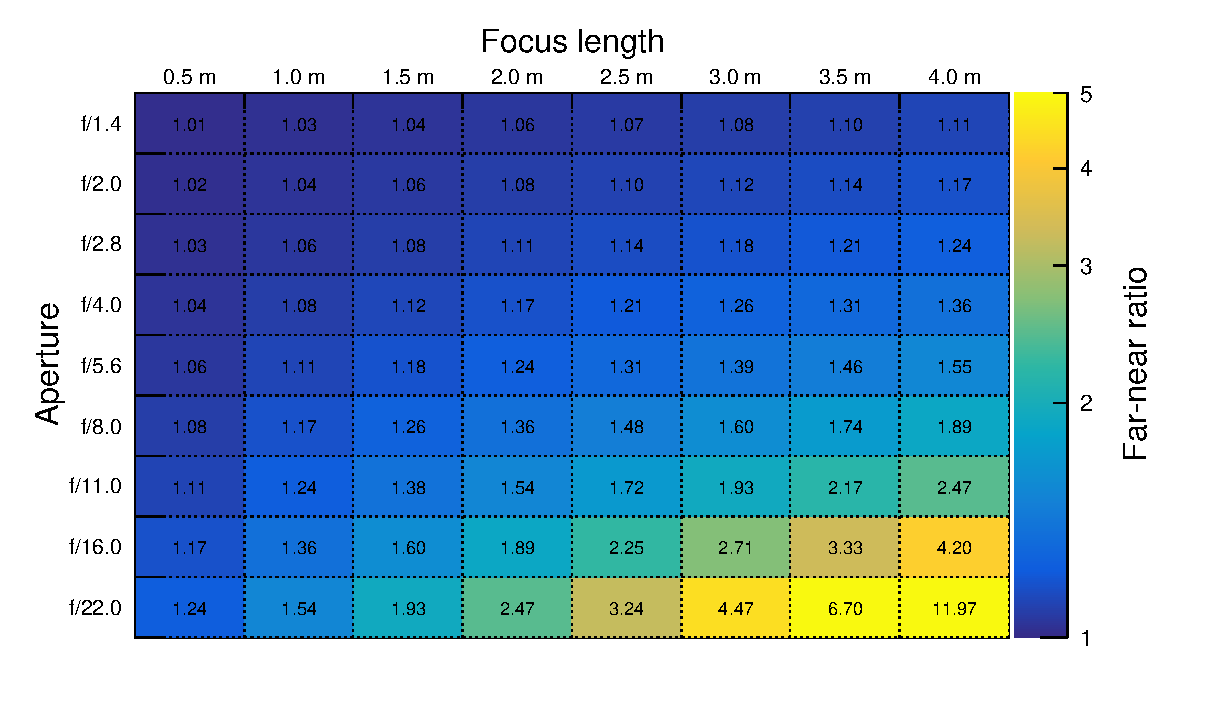
\includegraphics[center,width=0.78\textwidth]{img/far-near-ratio_focl40.eps}
\end{frame}

\begin{frame}[plain]{}
  \vspace{1ex}
  \centering
  Far-Near ratio | {\bf Focal length = 50 mm} |  Sony $\alpha$\hspace{0.1em}6000 (aps-c) | CoC = 0.036 mm
  
  \includegraphics[center,width=0.78\textwidth]{img/far-near-ratio_focl50.eps}
\end{frame}

\begin{frame}[plain]{}
  \vspace{1ex}
  \centering
  Far-Near ratio | {\bf Focal length = 100 mm} |  Sony $\alpha$\hspace{0.1em}6000 (aps-c) | CoC = 0.036 mm
  
  \includegraphics[center,width=0.78\textwidth]{img/far-near-ratio_focl100.eps}
\end{frame}

\begin{frame}[plain]{}
  \vspace{1ex}
  \centering
  Far-Near ratio | {\bf Focal length = 210 mm} |  Sony $\alpha$\hspace{0.1em}6000 (aps-c) | CoC = 0.036 mm
  
  \includegraphics[center,width=0.78\textwidth]{img/far-near-ratio_focl210.eps}
\end{frame}

\end{document}
